\documentclass[1p]{elsarticle_modified}
%\bibliographystyle{elsarticle-num}

%\usepackage[colorlinks]{hyperref}
%\usepackage{abbrmath_seonhwa} %\Abb, \Ascr, \Acal ,\Abf, \Afrak
\usepackage{amsfonts}
\usepackage{amssymb}
\usepackage{amsmath}
\usepackage{amsthm}
\usepackage{scalefnt}
\usepackage{amsbsy}
\usepackage{kotex}
\usepackage{caption}
\usepackage{subfig}
\usepackage{color}
\usepackage{graphicx}
\usepackage{xcolor} %% white, black, red, green, blue, cyan, magenta, yellow
\usepackage{float}
\usepackage{setspace}
\usepackage{hyperref}

\usepackage{tikz}
\usetikzlibrary{arrows}

\usepackage{multirow}
\usepackage{array} % fixed length table
\usepackage{hhline}

%%%%%%%%%%%%%%%%%%%%%
\makeatletter
\renewcommand*\env@matrix[1][\arraystretch]{%
	\edef\arraystretch{#1}%
	\hskip -\arraycolsep
	\let\@ifnextchar\new@ifnextchar
	\array{*\c@MaxMatrixCols c}}
\makeatother %https://tex.stackexchange.com/questions/14071/how-can-i-increase-the-line-spacing-in-a-matrix
%%%%%%%%%%%%%%%

\usepackage[normalem]{ulem}

\newcommand{\msout}[1]{\ifmmode\text{\sout{\ensuremath{#1}}}\else\sout{#1}\fi}
%SOURCE: \msout is \stkout macro in https://tex.stackexchange.com/questions/20609/strikeout-in-math-mode

\newcommand{\cancel}[1]{
	\ifmmode
	{\color{red}\msout{#1}}
	\else
	{\color{red}\sout{#1}}
	\fi
}

\newcommand{\add}[1]{
	{\color{blue}\uwave{#1}}
}

\newcommand{\replace}[2]{
	\ifmmode
	{\color{red}\msout{#1}}{\color{blue}\uwave{#2}}
	\else
	{\color{red}\sout{#1}}{\color{blue}\uwave{#2}}
	\fi
}

\newcommand{\Sol}{\mathcal{S}} %segment
\newcommand{\D}{D} %diagram
\newcommand{\A}{\mathcal{A}} %arc


%%%%%%%%%%%%%%%%%%%%%%%%%%%%%5 test

\def\sl{\operatorname{\textup{SL}}(2,\Cbb)}
\def\psl{\operatorname{\textup{PSL}}(2,\Cbb)}
\def\quan{\mkern 1mu \triangleright \mkern 1mu}

\theoremstyle{definition}
\newtheorem{thm}{Theorem}[section]
\newtheorem{prop}[thm]{Proposition}
\newtheorem{lem}[thm]{Lemma}
\newtheorem{ques}[thm]{Question}
\newtheorem{cor}[thm]{Corollary}
\newtheorem{defn}[thm]{Definition}
\newtheorem{exam}[thm]{Example}
\newtheorem{rmk}[thm]{Remark}
\newtheorem{alg}[thm]{Algorithm}

\newcommand{\I}{\sqrt{-1}}
\begin{document}

%\begin{frontmatter}
%
%\title{Boundary parabolic representations of knots up to 8 crossings}
%
%%% Group authors per affiliation:
%\author{Yunhi Cho} 
%\address{Department of Mathematics, University of Seoul, Seoul, Korea}
%\ead{yhcho@uos.ac.kr}
%
%
%\author{Seonhwa Kim} %\fnref{s_kim}}
%\address{Center for Geometry and Physics, Institute for Basic Science, Pohang, 37673, Korea}
%\ead{ryeona17@ibs.re.kr}
%
%\author{Hyuk Kim}
%\address{Department of Mathematical Sciences, Seoul National University, Seoul 08826, Korea}
%\ead{hyukkim@snu.ac.kr}
%
%\author{Seokbeom Yoon}
%\address{Department of Mathematical Sciences, Seoul National University, Seoul, 08826,  Korea}
%\ead{sbyoon15@snu.ac.kr}
%
%\begin{abstract}
%We find all boundary parabolic representation of knots up to 8 crossings.
%
%\end{abstract}
%\begin{keyword}
%    \MSC[2010] 57M25 
%\end{keyword}
%
%\end{frontmatter}

%\linenumbers
%\tableofcontents
%
\newcommand\colored[1]{\textcolor{white}{\rule[-0.35ex]{0.8em}{1.4ex}}\kern-0.8em\color{red} #1}%
%\newcommand\colored[1]{\textcolor{white}{ #1}\kern-2.17ex	\textcolor{white}{ #1}\kern-1.81ex	\textcolor{white}{ #1}\kern-2.15ex\color{red}#1	}

{\Large $\underline{12a_{0006}~(K12a_{0006})}$}

\setlength{\tabcolsep}{10pt}
\renewcommand{\arraystretch}{1.6}
\vspace{1cm}\begin{tabular}{m{100pt}>{\centering\arraybackslash}m{274pt}}
\multirow{5}{120pt}{
	\centering
	\includegraphics[width=112pt]{../../../GIT/diagram.site/Diagrams/png/807_12a_0006.png}\\
\ \ \ A knot diagram\footnotemark}&
\allowdisplaybreaks
\textbf{Linearized knot diagam} \\
\cline{2-2}
 &
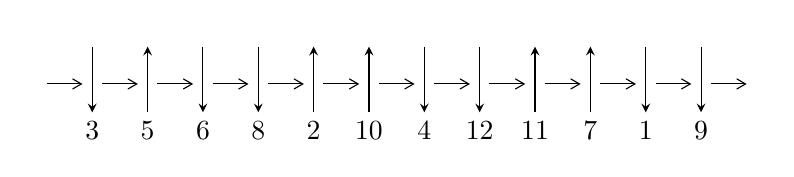
\begin{tikzpicture}[x=20pt, y=17pt]
	% nodes
	\node (C0) at (0, 0) {};
	\node (C1) at (1, 0) {};
	\node (C1U) at (1, +1) {};
	\node (C1D) at (1, -1) {3};

	\node (C2) at (2, 0) {};
	\node (C2U) at (2, +1) {};
	\node (C2D) at (2, -1) {5};

	\node (C3) at (3, 0) {};
	\node (C3U) at (3, +1) {};
	\node (C3D) at (3, -1) {6};

	\node (C4) at (4, 0) {};
	\node (C4U) at (4, +1) {};
	\node (C4D) at (4, -1) {8};

	\node (C5) at (5, 0) {};
	\node (C5U) at (5, +1) {};
	\node (C5D) at (5, -1) {2};

	\node (C6) at (6, 0) {};
	\node (C6U) at (6, +1) {};
	\node (C6D) at (6, -1) {10};

	\node (C7) at (7, 0) {};
	\node (C7U) at (7, +1) {};
	\node (C7D) at (7, -1) {4};

	\node (C8) at (8, 0) {};
	\node (C8U) at (8, +1) {};
	\node (C8D) at (8, -1) {12};

	\node (C9) at (9, 0) {};
	\node (C9U) at (9, +1) {};
	\node (C9D) at (9, -1) {11};

	\node (C10) at (10, 0) {};
	\node (C10U) at (10, +1) {};
	\node (C10D) at (10, -1) {7};

	\node (C11) at (11, 0) {};
	\node (C11U) at (11, +1) {};
	\node (C11D) at (11, -1) {1};

	\node (C12) at (12, 0) {};
	\node (C12U) at (12, +1) {};
	\node (C12D) at (12, -1) {9};
	\node (C13) at (13, 0) {};

	% arrows
	\draw[->,>={angle 60}]
	(C0) edge (C1) (C1) edge (C2) (C2) edge (C3) (C3) edge (C4) (C4) edge (C5) (C5) edge (C6) (C6) edge (C7) (C7) edge (C8) (C8) edge (C9) (C9) edge (C10) (C10) edge (C11) (C11) edge (C12) (C12) edge (C13) ;	\draw[->,>=stealth]
	(C1U) edge (C1D) (C2D) edge (C2U) (C3U) edge (C3D) (C4U) edge (C4D) (C5D) edge (C5U) (C6D) edge (C6U) (C7U) edge (C7D) (C8U) edge (C8D) (C9D) edge (C9U) (C10D) edge (C10U) (C11U) edge (C11D) (C12U) edge (C12D) ;
	\end{tikzpicture} \\
\hhline{~~} \\& 
\textbf{Solving Sequence} \\ \cline{2-2} 
 &
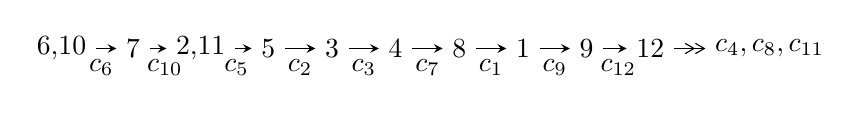
\begin{tikzpicture}[x=23pt, y=7pt]
	% node
	\node (A0) at (-1/8, 0) {6,10};
	\node (A1) at (1, 0) {7};
	\node (A2) at (33/16, 0) {2,11};
	\node (A3) at (25/8, 0) {5};
	\node (A4) at (33/8, 0) {3};
	\node (A5) at (41/8, 0) {4};
	\node (A6) at (49/8, 0) {8};
	\node (A7) at (57/8, 0) {1};
	\node (A8) at (65/8, 0) {9};
	\node (A9) at (73/8, 0) {12};
	\node (C1) at (1/2, -1) {$c_{6}$};
	\node (C2) at (3/2, -1) {$c_{10}$};
	\node (C3) at (21/8, -1) {$c_{5}$};
	\node (C4) at (29/8, -1) {$c_{2}$};
	\node (C5) at (37/8, -1) {$c_{3}$};
	\node (C6) at (45/8, -1) {$c_{7}$};
	\node (C7) at (53/8, -1) {$c_{1}$};
	\node (C8) at (61/8, -1) {$c_{9}$};
	\node (C9) at (69/8, -1) {$c_{12}$};
	\node (A10) at (11, 0) {$c_{4},c_{8},c_{11}$};

	% edge
	\draw[->,>=stealth]	
	(A0) edge (A1) (A1) edge (A2) (A2) edge (A3) (A3) edge (A4) (A4) edge (A5) (A5) edge (A6) (A6) edge (A7) (A7) edge (A8) (A8) edge (A9) ;
	\draw[->>,>={angle 60}]	
	(A9) edge (A10);
\end{tikzpicture} \\ 

\end{tabular} \\

\footnotetext{
The image of knot diagram is generated by the software ``\textbf{Draw programme}" developed by Andrew Bartholomew(\url{http://www.layer8.co.uk/maths/draw/index.htm\#Running-draw}), where we modified some parts for our purpose(\url{https://github.com/CATsTAILs/LinksPainter}).
}\phantom \\ \newline 
\centering \textbf{Ideals for irreducible components\footnotemark of $X_{\text{par}}$} 
 
\begin{align*}
I^u_{1}&=\langle 
-7.65110\times10^{246} u^{117}+2.10342\times10^{247} u^{116}+\cdots+7.39617\times10^{247} b-4.75087\times10^{248},\\
\phantom{I^u_{1}}&\phantom{= \langle  }-7.08530\times10^{247} u^{117}+1.80151\times10^{248} u^{116}+\cdots+4.43770\times10^{248} a-1.26778\times10^{249},\\
\phantom{I^u_{1}}&\phantom{= \langle  }u^{118}-3 u^{117}+\cdots-32 u+32\rangle \\
I^u_{2}&=\langle 
u^4 a- u^3 a+u^4- u^3+a u+b- a+u-1,\\
\phantom{I^u_{2}}&\phantom{= \langle  }- u^5 a+2 u^5+2 u^3 a-2 u^4- u^2 a-3 u^3+a^2-2 a u+4 u^2+2 a+2 u-2,\;u^6- u^5- u^4+2 u^3- u+1\rangle \\
\\
I^v_{1}&=\langle 
a,\;-3 v^4+4 v^3-10 v^2+b-21 v-7,\;v^5- v^4+3 v^3+8 v^2+5 v+1\rangle \\
\end{align*}
\raggedright * 3 irreducible components of $\dim_{\mathbb{C}}=0$, with total 135 representations.\\
\footnotetext{All coefficients of polynomials are rational numbers. But the coefficients are sometimes approximated in decimal forms when there is not enough margin.}
\newpage
\renewcommand{\arraystretch}{1}
\centering \section*{I. $I^u_{1}= \langle -7.65\times10^{246} u^{117}+2.10\times10^{247} u^{116}+\cdots+7.40\times10^{247} b-4.75\times10^{248},\;-7.09\times10^{247} u^{117}+1.80\times10^{248} u^{116}+\cdots+4.44\times10^{248} a-1.27\times10^{249},\;u^{118}-3 u^{117}+\cdots-32 u+32 \rangle$}
\flushleft \textbf{(i) Arc colorings}\\
\begin{tabular}{m{7pt} m{180pt} m{7pt} m{180pt} }
\flushright $a_{6}=$&$\begin{pmatrix}1\\0\end{pmatrix}$ \\
\flushright $a_{10}=$&$\begin{pmatrix}0\\u\end{pmatrix}$ \\
\flushright $a_{7}=$&$\begin{pmatrix}1\\- u^2\end{pmatrix}$ \\
\flushright $a_{2}=$&$\begin{pmatrix}0.159661 u^{117}-0.405956 u^{116}+\cdots-50.6753 u+2.85683\\0.103447 u^{117}-0.284393 u^{116}+\cdots-22.6938 u+6.42342\end{pmatrix}$ \\
\flushright $a_{11}=$&$\begin{pmatrix}u\\- u^3+u\end{pmatrix}$ \\
\flushright $a_{5}=$&$\begin{pmatrix}0.489272 u^{117}-1.92202 u^{116}+\cdots-100.177 u+40.5651\\0.340316 u^{117}-1.27077 u^{116}+\cdots-47.3105 u+17.7814\end{pmatrix}$ \\
\flushright $a_{3}=$&$\begin{pmatrix}-0.758810 u^{117}+2.70567 u^{116}+\cdots+104.493 u-38.0247\\-0.704038 u^{117}+2.56247 u^{116}+\cdots+117.303 u-43.3608\end{pmatrix}$ \\
\flushright $a_{4}=$&$\begin{pmatrix}-0.0547723 u^{117}+0.143196 u^{116}+\cdots-12.8108 u+5.33612\\-0.704038 u^{117}+2.56247 u^{116}+\cdots+117.303 u-43.3608\end{pmatrix}$ \\
\flushright $a_{8}=$&$\begin{pmatrix}-0.0350744 u^{117}+0.212518 u^{116}+\cdots-0.864347 u-4.50525\\0.0107154 u^{117}-0.0648548 u^{116}+\cdots-13.9025 u+5.51561\end{pmatrix}$ \\
\flushright $a_{1}=$&$\begin{pmatrix}-0.0588332 u^{117}+0.244742 u^{116}+\cdots+8.48235 u-6.58741\\-0.0237588 u^{117}+0.0322234 u^{116}+\cdots+9.34669 u-2.08216\end{pmatrix}$ \\
\flushright $a_{9}=$&$\begin{pmatrix}- u^3\\u^5- u^3+u\end{pmatrix}$ \\
\flushright $a_{12}=$&$\begin{pmatrix}-0.0347330 u^{117}+0.229528 u^{116}+\cdots+10.9263 u-7.78172\\0.0194075 u^{117}-0.0731735 u^{116}+\cdots+7.91588 u-1.10392\end{pmatrix}$\\&\end{tabular}
\flushleft \textbf{(ii) Obstruction class $= -1$}\\~\\
\flushleft \textbf{(iii) Cusp Shapes $= 1.13497 u^{117}-4.19176 u^{116}+\cdots-276.130 u+125.354$}\\~\\
\newpage\renewcommand{\arraystretch}{1}
\flushleft \textbf{(iv) u-Polynomials at the component}\newline \\
\begin{tabular}{m{50pt}|m{274pt}}
Crossings & \hspace{64pt}u-Polynomials at each crossing \\
\hline $$\begin{aligned}c_{1}\end{aligned}$$&$\begin{aligned}
&u^{118}+60 u^{117}+\cdots+8 u+1
\end{aligned}$\\
\hline $$\begin{aligned}c_{2},c_{5}\end{aligned}$$&$\begin{aligned}
&u^{118}+8 u^{117}+\cdots+8 u+1
\end{aligned}$\\
\hline $$\begin{aligned}c_{3}\end{aligned}$$&$\begin{aligned}
&u^{118}-8 u^{117}+\cdots-20012 u+337
\end{aligned}$\\
\hline $$\begin{aligned}c_{4},c_{7}\end{aligned}$$&$\begin{aligned}
&u^{118}+2 u^{117}+\cdots-8192 u-4096
\end{aligned}$\\
\hline $$\begin{aligned}c_{6},c_{10}\end{aligned}$$&$\begin{aligned}
&u^{118}-3 u^{117}+\cdots-32 u+32
\end{aligned}$\\
\hline $$\begin{aligned}c_{8},c_{12}\end{aligned}$$&$\begin{aligned}
&u^{118}-8 u^{117}+\cdots-2 u-1
\end{aligned}$\\
\hline $$\begin{aligned}c_{9}\end{aligned}$$&$\begin{aligned}
&u^{118}-39 u^{117}+\cdots-22016 u+1024
\end{aligned}$\\
\hline $$\begin{aligned}c_{11}\end{aligned}$$&$\begin{aligned}
&u^{118}+64 u^{117}+\cdots+46 u+1
\end{aligned}$\\
\hline
\end{tabular}\\~\\
\newpage\renewcommand{\arraystretch}{1}
\flushleft \textbf{(v) Riley Polynomials at the component}\newline \\
\begin{tabular}{m{50pt}|m{274pt}}
Crossings & \hspace{64pt}Riley Polynomials at each crossing \\
\hline $$\begin{aligned}c_{1}\end{aligned}$$&$\begin{aligned}
&y^{118}+4 y^{117}+\cdots-48 y+1
\end{aligned}$\\
\hline $$\begin{aligned}c_{2},c_{5}\end{aligned}$$&$\begin{aligned}
&y^{118}+60 y^{117}+\cdots+8 y+1
\end{aligned}$\\
\hline $$\begin{aligned}c_{3}\end{aligned}$$&$\begin{aligned}
&y^{118}-52 y^{117}+\cdots+347123352 y+113569
\end{aligned}$\\
\hline $$\begin{aligned}c_{4},c_{7}\end{aligned}$$&$\begin{aligned}
&y^{118}-70 y^{117}+\cdots-285212672 y+16777216
\end{aligned}$\\
\hline $$\begin{aligned}c_{6},c_{10}\end{aligned}$$&$\begin{aligned}
&y^{118}-39 y^{117}+\cdots-22016 y+1024
\end{aligned}$\\
\hline $$\begin{aligned}c_{8},c_{12}\end{aligned}$$&$\begin{aligned}
&y^{118}-64 y^{117}+\cdots-46 y+1
\end{aligned}$\\
\hline $$\begin{aligned}c_{9}\end{aligned}$$&$\begin{aligned}
&y^{118}+73 y^{117}+\cdots-33161216 y+1048576
\end{aligned}$\\
\hline $$\begin{aligned}c_{11}\end{aligned}$$&$\begin{aligned}
&y^{118}-12 y^{117}+\cdots+1158 y+1
\end{aligned}$\\
\hline
\end{tabular}\\~\\
\newpage\flushleft \textbf{(vi) Complex Volumes and Cusp Shapes}
$$\begin{array}{c|c|c}  
\text{Solutions to }I^u_{1}& \I (\text{vol} + \sqrt{-1}CS) & \text{Cusp shape}\\
 \hline 
\begin{aligned}
u &= -0.057111 + 0.994719 I \\
a &= \phantom{-}0.36450 - 1.63146 I \\
b &= -0.479763 - 1.116650 I\end{aligned}
 & -3.79426 + 5.91242 I & \phantom{-0.000000 } 0 \\ \hline\begin{aligned}
u &= -0.057111 - 0.994719 I \\
a &= \phantom{-}0.36450 + 1.63146 I \\
b &= -0.479763 + 1.116650 I\end{aligned}
 & -3.79426 - 5.91242 I & \phantom{-0.000000 } 0 \\ \hline\begin{aligned}
u &= -0.914029 + 0.393303 I \\
a &= \phantom{-}0.297266 - 1.272970 I \\
b &= -0.004632 - 0.992140 I\end{aligned}
 & -1.56812 - 4.24852 I & \phantom{-0.000000 } 0 \\ \hline\begin{aligned}
u &= -0.914029 - 0.393303 I \\
a &= \phantom{-}0.297266 + 1.272970 I \\
b &= -0.004632 + 0.992140 I\end{aligned}
 & -1.56812 + 4.24852 I & \phantom{-0.000000 } 0 \\ \hline\begin{aligned}
u &= -0.641087 + 0.760665 I \\
a &= \phantom{-}0.779065 - 0.477001 I \\
b &= \phantom{-}0.509907 - 0.068037 I\end{aligned}
 & -2.44908 + 1.22370 I & \phantom{-0.000000 } 0 \\ \hline\begin{aligned}
u &= -0.641087 - 0.760665 I \\
a &= \phantom{-}0.779065 + 0.477001 I \\
b &= \phantom{-}0.509907 + 0.068037 I\end{aligned}
 & -2.44908 - 1.22370 I & \phantom{-0.000000 } 0 \\ \hline\begin{aligned}
u &= -0.849815 + 0.541103 I \\
a &= -0.268387 - 0.139659 I \\
b &= \phantom{-}0.674649 + 0.872777 I\end{aligned}
 & \phantom{-}0.565713 + 0.424578 I & \phantom{-0.000000 } 0 \\ \hline\begin{aligned}
u &= -0.849815 - 0.541103 I \\
a &= -0.268387 + 0.139659 I \\
b &= \phantom{-}0.674649 - 0.872777 I\end{aligned}
 & \phantom{-}0.565713 - 0.424578 I & \phantom{-0.000000 } 0 \\ \hline\begin{aligned}
u &= -0.991085 + 0.050636 I \\
a &= -1.44835 + 0.47132 I \\
b &= \phantom{-}0.610150 + 0.985347 I\end{aligned}
 & \phantom{-}2.32252 + 1.20341 I & \phantom{-0.000000 } 0 \\ \hline\begin{aligned}
u &= -0.991085 - 0.050636 I \\
a &= -1.44835 - 0.47132 I \\
b &= \phantom{-}0.610150 - 0.985347 I\end{aligned}
 & \phantom{-}2.32252 - 1.20341 I & \phantom{-0.000000 } 0\\
 \hline 
 \end{array}$$\newpage$$\begin{array}{c|c|c}  
\text{Solutions to }I^u_{1}& \I (\text{vol} + \sqrt{-1}CS) & \text{Cusp shape}\\
 \hline 
\begin{aligned}
u &= \phantom{-}0.750948 + 0.648450 I \\
a &= \phantom{-}0.52003 - 2.23767 I \\
b &= \phantom{-}0.403810 - 1.096830 I\end{aligned}
 & -1.81430 - 1.19890 I & \phantom{-0.000000 } 0 \\ \hline\begin{aligned}
u &= \phantom{-}0.750948 - 0.648450 I \\
a &= \phantom{-}0.52003 + 2.23767 I \\
b &= \phantom{-}0.403810 + 1.096830 I\end{aligned}
 & -1.81430 + 1.19890 I & \phantom{-0.000000 } 0 \\ \hline\begin{aligned}
u &= \phantom{-}0.704841 + 0.728643 I \\
a &= -1.42404 + 1.25197 I \\
b &= \phantom{-}0.687054 + 0.817693 I\end{aligned}
 & -3.03391 + 1.35788 I & \phantom{-0.000000 } 0 \\ \hline\begin{aligned}
u &= \phantom{-}0.704841 - 0.728643 I \\
a &= -1.42404 - 1.25197 I \\
b &= \phantom{-}0.687054 - 0.817693 I\end{aligned}
 & -3.03391 - 1.35788 I & \phantom{-0.000000 } 0 \\ \hline\begin{aligned}
u &= -0.595125 + 0.821259 I \\
a &= -0.192234 + 0.242458 I \\
b &= -0.804532 + 0.208505 I\end{aligned}
 & -3.00739 + 1.82099 I & \phantom{-0.000000 } 0 \\ \hline\begin{aligned}
u &= -0.595125 - 0.821259 I \\
a &= -0.192234 - 0.242458 I \\
b &= -0.804532 - 0.208505 I\end{aligned}
 & -3.00739 - 1.82099 I & \phantom{-0.000000 } 0 \\ \hline\begin{aligned}
u &= -0.242106 + 0.999487 I \\
a &= \phantom{-}0.49124 + 1.66110 I \\
b &= -0.423992 + 1.099160 I\end{aligned}
 & -4.22546 - 1.56777 I & \phantom{-0.000000 } 0 \\ \hline\begin{aligned}
u &= -0.242106 - 0.999487 I \\
a &= \phantom{-}0.49124 - 1.66110 I \\
b &= -0.423992 - 1.099160 I\end{aligned}
 & -4.22546 + 1.56777 I & \phantom{-0.000000 } 0 \\ \hline\begin{aligned}
u &= \phantom{-}0.761083 + 0.704310 I \\
a &= \phantom{-}0.18432 + 1.73897 I \\
b &= -0.534333 + 1.210310 I\end{aligned}
 & -9.66639 - 3.23714 I & \phantom{-0.000000 } 0 \\ \hline\begin{aligned}
u &= \phantom{-}0.761083 - 0.704310 I \\
a &= \phantom{-}0.18432 - 1.73897 I \\
b &= -0.534333 - 1.210310 I\end{aligned}
 & -9.66639 + 3.23714 I & \phantom{-0.000000 } 0\\
 \hline 
 \end{array}$$\newpage$$\begin{array}{c|c|c}  
\text{Solutions to }I^u_{1}& \I (\text{vol} + \sqrt{-1}CS) & \text{Cusp shape}\\
 \hline 
\begin{aligned}
u &= \phantom{-}1.026530 + 0.206251 I \\
a &= -1.70974 + 1.21108 I \\
b &= \phantom{-}0.573243 + 1.038280 I\end{aligned}
 & \phantom{-}1.95085 + 5.61000 I & \phantom{-0.000000 } 0 \\ \hline\begin{aligned}
u &= \phantom{-}1.026530 - 0.206251 I \\
a &= -1.70974 - 1.21108 I \\
b &= \phantom{-}0.573243 - 1.038280 I\end{aligned}
 & \phantom{-}1.95085 - 5.61000 I & \phantom{-0.000000 } 0 \\ \hline\begin{aligned}
u &= \phantom{-}0.667456 + 0.812256 I \\
a &= \phantom{-}0.291954 + 0.052077 I \\
b &= \phantom{-}0.700820 - 0.783953 I\end{aligned}
 & -2.93079 - 3.91418 I & \phantom{-0.000000 } 0 \\ \hline\begin{aligned}
u &= \phantom{-}0.667456 - 0.812256 I \\
a &= \phantom{-}0.291954 - 0.052077 I \\
b &= \phantom{-}0.700820 + 0.783953 I\end{aligned}
 & -2.93079 + 3.91418 I & \phantom{-0.000000 } 0 \\ \hline\begin{aligned}
u &= -0.441663 + 0.835178 I \\
a &= \phantom{-}0.448495 - 0.613915 I \\
b &= -0.185637 - 0.547949 I\end{aligned}
 & -2.01865 + 1.48429 I & \phantom{-0.000000 } 0 \\ \hline\begin{aligned}
u &= -0.441663 - 0.835178 I \\
a &= \phantom{-}0.448495 + 0.613915 I \\
b &= -0.185637 + 0.547949 I\end{aligned}
 & -2.01865 - 1.48429 I & \phantom{-0.000000 } 0 \\ \hline\begin{aligned}
u &= \phantom{-}1.054750 + 0.101458 I \\
a &= -0.158985 + 0.740344 I \\
b &= \phantom{-}0.645223 - 0.470242 I\end{aligned}
 & \phantom{-}3.58808 + 0.84208 I & \phantom{-0.000000 } 0 \\ \hline\begin{aligned}
u &= \phantom{-}1.054750 - 0.101458 I \\
a &= -0.158985 - 0.740344 I \\
b &= \phantom{-}0.645223 + 0.470242 I\end{aligned}
 & \phantom{-}3.58808 - 0.84208 I & \phantom{-0.000000 } 0 \\ \hline\begin{aligned}
u &= -1.056930 + 0.134697 I \\
a &= -0.653037 + 0.468905 I \\
b &= \phantom{-}0.679183 - 0.575083 I\end{aligned}
 & \phantom{-}3.51464 - 3.77326 I & \phantom{-0.000000 } 0 \\ \hline\begin{aligned}
u &= -1.056930 - 0.134697 I \\
a &= -0.653037 - 0.468905 I \\
b &= \phantom{-}0.679183 + 0.575083 I\end{aligned}
 & \phantom{-}3.51464 + 3.77326 I & \phantom{-0.000000 } 0\\
 \hline 
 \end{array}$$\newpage$$\begin{array}{c|c|c}  
\text{Solutions to }I^u_{1}& \I (\text{vol} + \sqrt{-1}CS) & \text{Cusp shape}\\
 \hline 
\begin{aligned}
u &= -0.574725 + 0.902696 I \\
a &= \phantom{-}0.21041 - 1.67524 I \\
b &= -0.538247 - 1.172420 I\end{aligned}
 & -5.84550 + 6.78193 I & \phantom{-0.000000 } 0 \\ \hline\begin{aligned}
u &= -0.574725 - 0.902696 I \\
a &= \phantom{-}0.21041 + 1.67524 I \\
b &= -0.538247 + 1.172420 I\end{aligned}
 & -5.84550 - 6.78193 I & \phantom{-0.000000 } 0 \\ \hline\begin{aligned}
u &= \phantom{-}0.926136 + 0.543311 I \\
a &= \phantom{-}0.583704 + 0.628251 I \\
b &= \phantom{-}0.581906 - 0.193380 I\end{aligned}
 & \phantom{-}1.35120 + 2.05184 I & \phantom{-0.000000 } 0 \\ \hline\begin{aligned}
u &= \phantom{-}0.926136 - 0.543311 I \\
a &= \phantom{-}0.583704 - 0.628251 I \\
b &= \phantom{-}0.581906 + 0.193380 I\end{aligned}
 & \phantom{-}1.35120 - 2.05184 I & \phantom{-0.000000 } 0 \\ \hline\begin{aligned}
u &= \phantom{-}0.817393 + 0.699752 I \\
a &= -0.274441 - 0.202673 I \\
b &= -0.874488 - 0.173434 I\end{aligned}
 & -6.53571 + 1.89043 I & \phantom{-0.000000 } 0 \\ \hline\begin{aligned}
u &= \phantom{-}0.817393 - 0.699752 I \\
a &= -0.274441 + 0.202673 I \\
b &= -0.874488 + 0.173434 I\end{aligned}
 & -6.53571 - 1.89043 I & \phantom{-0.000000 } 0 \\ \hline\begin{aligned}
u &= -0.918223 + 0.103095 I \\
a &= \phantom{-}0.860492 + 1.120820 I \\
b &= -0.448856 - 1.120990 I\end{aligned}
 & -5.56593 + 3.83415 I & \phantom{-0.000000 } 0 \\ \hline\begin{aligned}
u &= -0.918223 - 0.103095 I \\
a &= \phantom{-}0.860492 - 1.120820 I \\
b &= -0.448856 + 1.120990 I\end{aligned}
 & -5.56593 - 3.83415 I & \phantom{-0.000000 } 0 \\ \hline\begin{aligned}
u &= -0.790275 + 0.740752 I \\
a &= -1.51469 - 2.91008 I \\
b &= \phantom{-}0.439874 - 1.114530 I\end{aligned}
 & -5.31904 - 2.44166 I & \phantom{-0.000000 } 0 \\ \hline\begin{aligned}
u &= -0.790275 - 0.740752 I \\
a &= -1.51469 + 2.91008 I \\
b &= \phantom{-}0.439874 + 1.114530 I\end{aligned}
 & -5.31904 + 2.44166 I & \phantom{-0.000000 } 0\\
 \hline 
 \end{array}$$\newpage$$\begin{array}{c|c|c}  
\text{Solutions to }I^u_{1}& \I (\text{vol} + \sqrt{-1}CS) & \text{Cusp shape}\\
 \hline 
\begin{aligned}
u &= -0.938249 + 0.587408 I \\
a &= -1.164570 - 0.579553 I \\
b &= \phantom{-}0.718691 - 0.741494 I\end{aligned}
 & \phantom{-}0.95583 - 4.87112 I & \phantom{-0.000000 } 0 \\ \hline\begin{aligned}
u &= -0.938249 - 0.587408 I \\
a &= -1.164570 + 0.579553 I \\
b &= \phantom{-}0.718691 + 0.741494 I\end{aligned}
 & \phantom{-}0.95583 + 4.87112 I & \phantom{-0.000000 } 0 \\ \hline\begin{aligned}
u &= -0.712579 + 0.849832 I \\
a &= \phantom{-}0.51391 + 2.00089 I \\
b &= -0.315907 + 1.207150 I\end{aligned}
 & -7.37780 - 1.81999 I & \phantom{-0.000000 } 0 \\ \hline\begin{aligned}
u &= -0.712579 - 0.849832 I \\
a &= \phantom{-}0.51391 - 2.00089 I \\
b &= -0.315907 - 1.207150 I\end{aligned}
 & -7.37780 + 1.81999 I & \phantom{-0.000000 } 0 \\ \hline\begin{aligned}
u &= -0.713912 + 0.864317 I \\
a &= \phantom{-}0.38520 + 2.30740 I \\
b &= \phantom{-}0.460796 + 1.118670 I\end{aligned}
 & -5.16425 + 5.15948 I & \phantom{-0.000000 } 0 \\ \hline\begin{aligned}
u &= -0.713912 - 0.864317 I \\
a &= \phantom{-}0.38520 - 2.30740 I \\
b &= \phantom{-}0.460796 - 1.118670 I\end{aligned}
 & -5.16425 - 5.15948 I & \phantom{-0.000000 } 0 \\ \hline\begin{aligned}
u &= \phantom{-}0.903754 + 0.685135 I \\
a &= -0.229534 - 1.073390 I \\
b &= -0.834503 + 0.236031 I\end{aligned}
 & -6.26654 + 3.43511 I & \phantom{-0.000000 } 0 \\ \hline\begin{aligned}
u &= \phantom{-}0.903754 - 0.685135 I \\
a &= -0.229534 + 1.073390 I \\
b &= -0.834503 - 0.236031 I\end{aligned}
 & -6.26654 - 3.43511 I & \phantom{-0.000000 } 0 \\ \hline\begin{aligned}
u &= -0.092158 + 0.857430 I \\
a &= \phantom{-}0.093803 + 0.222170 I \\
b &= -0.555039 + 0.193650 I\end{aligned}
 & -1.24389 + 1.74559 I & \phantom{-0.000000 } 0 \\ \hline\begin{aligned}
u &= -0.092158 - 0.857430 I \\
a &= \phantom{-}0.093803 - 0.222170 I \\
b &= -0.555039 - 0.193650 I\end{aligned}
 & -1.24389 - 1.74559 I & \phantom{-0.000000 } 0\\
 \hline 
 \end{array}$$\newpage$$\begin{array}{c|c|c}  
\text{Solutions to }I^u_{1}& \I (\text{vol} + \sqrt{-1}CS) & \text{Cusp shape}\\
 \hline 
\begin{aligned}
u &= \phantom{-}0.843744 + 0.765170 I \\
a &= \phantom{-}0.42452 - 2.02910 I \\
b &= -0.333480 - 1.250080 I\end{aligned}
 & -11.06080 + 5.93333 I & \phantom{-0.000000 } 0 \\ \hline\begin{aligned}
u &= \phantom{-}0.843744 - 0.765170 I \\
a &= \phantom{-}0.42452 + 2.02910 I \\
b &= -0.333480 + 1.250080 I\end{aligned}
 & -11.06080 - 5.93333 I & \phantom{-0.000000 } 0 \\ \hline\begin{aligned}
u &= \phantom{-}1.072050 + 0.405478 I \\
a &= \phantom{-}1.268290 - 0.321054 I \\
b &= -0.356382 - 0.560236 I\end{aligned}
 & \phantom{-}2.19895 + 1.79255 I & \phantom{-0.000000 } 0 \\ \hline\begin{aligned}
u &= \phantom{-}1.072050 - 0.405478 I \\
a &= \phantom{-}1.268290 + 0.321054 I \\
b &= -0.356382 + 0.560236 I\end{aligned}
 & \phantom{-}2.19895 - 1.79255 I & \phantom{-0.000000 } 0 \\ \hline\begin{aligned}
u &= \phantom{-}0.949358 + 0.655602 I \\
a &= -1.50109 + 2.42720 I \\
b &= \phantom{-}0.487936 + 1.117660 I\end{aligned}
 & -1.19730 + 6.30191 I & \phantom{-0.000000 } 0 \\ \hline\begin{aligned}
u &= \phantom{-}0.949358 - 0.655602 I \\
a &= -1.50109 - 2.42720 I \\
b &= \phantom{-}0.487936 - 1.117660 I\end{aligned}
 & -1.19730 - 6.30191 I & \phantom{-0.000000 } 0 \\ \hline\begin{aligned}
u &= \phantom{-}1.154880 + 0.081470 I \\
a &= \phantom{-}0.850435 - 0.258649 I \\
b &= -0.594989 + 0.390000 I\end{aligned}
 & \phantom{-}3.41320 + 0.71117 I & \phantom{-0.000000 } 0 \\ \hline\begin{aligned}
u &= \phantom{-}1.154880 - 0.081470 I \\
a &= \phantom{-}0.850435 + 0.258649 I \\
b &= -0.594989 - 0.390000 I\end{aligned}
 & \phantom{-}3.41320 - 0.71117 I & \phantom{-0.000000 } 0 \\ \hline\begin{aligned}
u &= \phantom{-}0.952170 + 0.675540 I \\
a &= \phantom{-}2.08030 - 1.86808 I \\
b &= -0.554021 - 1.178320 I\end{aligned}
 & -9.07220 + 8.55233 I & \phantom{-0.000000 } 0 \\ \hline\begin{aligned}
u &= \phantom{-}0.952170 - 0.675540 I \\
a &= \phantom{-}2.08030 + 1.86808 I \\
b &= -0.554021 + 1.178320 I\end{aligned}
 & -9.07220 - 8.55233 I & \phantom{-0.000000 } 0\\
 \hline 
 \end{array}$$\newpage$$\begin{array}{c|c|c}  
\text{Solutions to }I^u_{1}& \I (\text{vol} + \sqrt{-1}CS) & \text{Cusp shape}\\
 \hline 
\begin{aligned}
u &= -0.933711 + 0.711611 I \\
a &= \phantom{-}0.42213 + 2.16878 I \\
b &= \phantom{-}0.395467 + 1.151170 I\end{aligned}
 & -4.87773 - 3.09159 I & \phantom{-0.000000 } 0 \\ \hline\begin{aligned}
u &= -0.933711 - 0.711611 I \\
a &= \phantom{-}0.42213 - 2.16878 I \\
b &= \phantom{-}0.395467 - 1.151170 I\end{aligned}
 & -4.87773 + 3.09159 I & \phantom{-0.000000 } 0 \\ \hline\begin{aligned}
u &= \phantom{-}0.906410 + 0.760816 I \\
a &= -1.12132 + 1.34343 I \\
b &= -0.292550 + 1.220230 I\end{aligned}
 & -10.87470 - 0.17205 I & \phantom{-0.000000 } 0 \\ \hline\begin{aligned}
u &= \phantom{-}0.906410 - 0.760816 I \\
a &= -1.12132 - 1.34343 I \\
b &= -0.292550 - 1.220230 I\end{aligned}
 & -10.87470 + 0.17205 I & \phantom{-0.000000 } 0 \\ \hline\begin{aligned}
u &= \phantom{-}0.703346 + 0.968542 I \\
a &= -0.234705 - 0.299671 I \\
b &= -0.841845 - 0.256862 I\end{aligned}
 & -5.90980 - 6.28332 I & \phantom{-0.000000 } 0 \\ \hline\begin{aligned}
u &= \phantom{-}0.703346 - 0.968542 I \\
a &= -0.234705 + 0.299671 I \\
b &= -0.841845 + 0.256862 I\end{aligned}
 & -5.90980 + 6.28332 I & \phantom{-0.000000 } 0 \\ \hline\begin{aligned}
u &= \phantom{-}0.981963 + 0.689993 I \\
a &= -0.119645 - 0.167424 I \\
b &= \phantom{-}0.727220 - 0.874257 I\end{aligned}
 & -2.20059 + 4.08134 I & \phantom{-0.000000 } 0 \\ \hline\begin{aligned}
u &= \phantom{-}0.981963 - 0.689993 I \\
a &= -0.119645 + 0.167424 I \\
b &= \phantom{-}0.727220 + 0.874257 I\end{aligned}
 & -2.20059 - 4.08134 I & \phantom{-0.000000 } 0 \\ \hline\begin{aligned}
u &= -1.174600 + 0.288507 I \\
a &= \phantom{-}0.551612 + 0.463296 I \\
b &= -0.695913 - 0.362854 I\end{aligned}
 & \phantom{-}2.63779 - 5.83888 I & \phantom{-0.000000 } 0 \\ \hline\begin{aligned}
u &= -1.174600 - 0.288507 I \\
a &= \phantom{-}0.551612 - 0.463296 I \\
b &= -0.695913 + 0.362854 I\end{aligned}
 & \phantom{-}2.63779 + 5.83888 I & \phantom{-0.000000 } 0\\
 \hline 
 \end{array}$$\newpage$$\begin{array}{c|c|c}  
\text{Solutions to }I^u_{1}& \I (\text{vol} + \sqrt{-1}CS) & \text{Cusp shape}\\
 \hline 
\begin{aligned}
u &= \phantom{-}0.766573 + 0.949834 I \\
a &= \phantom{-}0.54077 - 2.08818 I \\
b &= -0.275600 - 1.221680 I\end{aligned}
 & -10.63780 - 2.75551 I & \phantom{-0.000000 } 0 \\ \hline\begin{aligned}
u &= \phantom{-}0.766573 - 0.949834 I \\
a &= \phantom{-}0.54077 + 2.08818 I \\
b &= -0.275600 + 1.221680 I\end{aligned}
 & -10.63780 + 2.75551 I & \phantom{-0.000000 } 0 \\ \hline\begin{aligned}
u &= \phantom{-}0.776994 + 0.041855 I \\
a &= \phantom{-}0.66142 - 1.68179 I \\
b &= \phantom{-}0.218885 - 1.009740 I\end{aligned}
 & -0.490861 - 0.714549 I & -2.00000 - 0.48683 I \\ \hline\begin{aligned}
u &= \phantom{-}0.776994 - 0.041855 I \\
a &= \phantom{-}0.66142 + 1.68179 I \\
b &= \phantom{-}0.218885 + 1.009740 I\end{aligned}
 & -0.490861 + 0.714549 I & -2.00000 + 0.48683 I \\ \hline\begin{aligned}
u &= -1.012390 + 0.692789 I \\
a &= \phantom{-}0.584170 - 0.489883 I \\
b &= \phantom{-}0.672262 + 0.132528 I\end{aligned}
 & -1.36149 - 6.75234 I & \phantom{-0.000000 } 0 \\ \hline\begin{aligned}
u &= -1.012390 - 0.692789 I \\
a &= \phantom{-}0.584170 + 0.489883 I \\
b &= \phantom{-}0.672262 - 0.132528 I\end{aligned}
 & -1.36149 + 6.75234 I & \phantom{-0.000000 } 0 \\ \hline\begin{aligned}
u &= -0.628903 + 0.449098 I \\
a &= \phantom{-}2.54132 - 0.00188 I \\
b &= \phantom{-}0.020939 + 0.603233 I\end{aligned}
 & -2.54168 + 0.64755 I & -6.08336 + 1.44392 I \\ \hline\begin{aligned}
u &= -0.628903 - 0.449098 I \\
a &= \phantom{-}2.54132 + 0.00188 I \\
b &= \phantom{-}0.020939 - 0.603233 I\end{aligned}
 & -2.54168 - 0.64755 I & -6.08336 - 1.44392 I \\ \hline\begin{aligned}
u &= \phantom{-}0.706770 + 1.008380 I \\
a &= \phantom{-}0.16558 + 1.66086 I \\
b &= -0.563795 + 1.176200 I\end{aligned}
 & -8.6542 - 11.4670 I & \phantom{-0.000000 } 0 \\ \hline\begin{aligned}
u &= \phantom{-}0.706770 - 1.008380 I \\
a &= \phantom{-}0.16558 - 1.66086 I \\
b &= -0.563795 - 1.176200 I\end{aligned}
 & -8.6542 + 11.4670 I & \phantom{-0.000000 } 0\\
 \hline 
 \end{array}$$\newpage$$\begin{array}{c|c|c}  
\text{Solutions to }I^u_{1}& \I (\text{vol} + \sqrt{-1}CS) & \text{Cusp shape}\\
 \hline 
\begin{aligned}
u &= \phantom{-}1.199720 + 0.314561 I \\
a &= \phantom{-}0.370854 + 0.093116 I \\
b &= -0.424562 + 1.045720 I\end{aligned}
 & \phantom{-}0.62638 - 1.63995 I & \phantom{-0.000000 } 0 \\ \hline\begin{aligned}
u &= \phantom{-}1.199720 - 0.314561 I \\
a &= \phantom{-}0.370854 - 0.093116 I \\
b &= -0.424562 - 1.045720 I\end{aligned}
 & \phantom{-}0.62638 + 1.63995 I & \phantom{-0.000000 } 0 \\ \hline\begin{aligned}
u &= \phantom{-}1.019770 + 0.714724 I \\
a &= -0.901138 + 0.757961 I \\
b &= \phantom{-}0.760109 + 0.761507 I\end{aligned}
 & -1.86733 + 9.65076 I & \phantom{-0.000000 } 0 \\ \hline\begin{aligned}
u &= \phantom{-}1.019770 - 0.714724 I \\
a &= -0.901138 - 0.757961 I \\
b &= \phantom{-}0.760109 - 0.761507 I\end{aligned}
 & -1.86733 - 9.65076 I & \phantom{-0.000000 } 0 \\ \hline\begin{aligned}
u &= -1.001870 + 0.750136 I \\
a &= -0.82058 - 1.37636 I \\
b &= -0.252783 - 1.215880 I\end{aligned}
 & -6.49755 - 4.12996 I & \phantom{-0.000000 } 0 \\ \hline\begin{aligned}
u &= -1.001870 - 0.750136 I \\
a &= -0.82058 + 1.37636 I \\
b &= -0.252783 + 1.215880 I\end{aligned}
 & -6.49755 + 4.12996 I & \phantom{-0.000000 } 0 \\ \hline\begin{aligned}
u &= \phantom{-}1.246440 + 0.134432 I \\
a &= \phantom{-}1.263590 - 0.327615 I \\
b &= -0.513444 - 1.082540 I\end{aligned}
 & \phantom{-}1.38319 + 5.13395 I & \phantom{-0.000000 } 0 \\ \hline\begin{aligned}
u &= \phantom{-}1.246440 - 0.134432 I \\
a &= \phantom{-}1.263590 + 0.327615 I \\
b &= -0.513444 + 1.082540 I\end{aligned}
 & \phantom{-}1.38319 - 5.13395 I & \phantom{-0.000000 } 0 \\ \hline\begin{aligned}
u &= -0.739637\phantom{ +0.000000I} \\
a &= \phantom{-}2.08237\phantom{ +0.000000I} \\
b &= -0.538572\phantom{ +0.000000I}\end{aligned}
 & -2.71088\phantom{ +0.000000I} & -0.754640\phantom{ +0.000000I} \\ \hline\begin{aligned}
u &= -1.050650 + 0.696469 I \\
a &= -0.151310 + 0.784583 I \\
b &= -0.842658 - 0.284149 I\end{aligned}
 & -1.65144 - 7.50770 I & \phantom{-0.000000 } 0\\
 \hline 
 \end{array}$$\newpage$$\begin{array}{c|c|c}  
\text{Solutions to }I^u_{1}& \I (\text{vol} + \sqrt{-1}CS) & \text{Cusp shape}\\
 \hline 
\begin{aligned}
u &= -1.050650 - 0.696469 I \\
a &= -0.151310 - 0.784583 I \\
b &= -0.842658 + 0.284149 I\end{aligned}
 & -1.65144 + 7.50770 I & \phantom{-0.000000 } 0 \\ \hline\begin{aligned}
u &= -1.021640 + 0.750308 I \\
a &= -1.24048 - 2.43396 I \\
b &= \phantom{-}0.490690 - 1.148020 I\end{aligned}
 & -4.20666 - 11.16730 I & \phantom{-0.000000 } 0 \\ \hline\begin{aligned}
u &= -1.021640 - 0.750308 I \\
a &= -1.24048 + 2.43396 I \\
b &= \phantom{-}0.490690 + 1.148020 I\end{aligned}
 & -4.20666 + 11.16730 I & \phantom{-0.000000 } 0 \\ \hline\begin{aligned}
u &= -1.115320 + 0.606056 I \\
a &= \phantom{-}1.230240 + 0.596883 I \\
b &= -0.351425 + 0.666628 I\end{aligned}
 & \phantom{-}0.06726 - 6.85727 I & \phantom{-0.000000 } 0 \\ \hline\begin{aligned}
u &= -1.115320 - 0.606056 I \\
a &= \phantom{-}1.230240 - 0.596883 I \\
b &= -0.351425 - 0.666628 I\end{aligned}
 & \phantom{-}0.06726 + 6.85727 I & \phantom{-0.000000 } 0 \\ \hline\begin{aligned}
u &= -1.178770 + 0.503879 I \\
a &= \phantom{-}0.134512 - 0.367275 I \\
b &= -0.373896 - 1.016460 I\end{aligned}
 & -1.02731 - 3.71542 I & \phantom{-0.000000 } 0 \\ \hline\begin{aligned}
u &= -1.178770 - 0.503879 I \\
a &= \phantom{-}0.134512 + 0.367275 I \\
b &= -0.373896 + 1.016460 I\end{aligned}
 & -1.02731 + 3.71542 I & \phantom{-0.000000 } 0 \\ \hline\begin{aligned}
u &= -1.244210 + 0.324599 I \\
a &= \phantom{-}1.48321 + 0.70609 I \\
b &= -0.542963 + 1.102660 I\end{aligned}
 & \phantom{-}0.46596 - 10.60320 I & \phantom{-0.000000 } 0 \\ \hline\begin{aligned}
u &= -1.244210 - 0.324599 I \\
a &= \phantom{-}1.48321 - 0.70609 I \\
b &= -0.542963 - 1.102660 I\end{aligned}
 & \phantom{-}0.46596 + 10.60320 I & \phantom{-0.000000 } 0 \\ \hline\begin{aligned}
u &= -1.085240 + 0.716483 I \\
a &= \phantom{-}1.69229 + 1.72293 I \\
b &= -0.574228 + 1.169280 I\end{aligned}
 & -4.29675 - 12.74330 I & \phantom{-0.000000 } 0\\
 \hline 
 \end{array}$$\newpage$$\begin{array}{c|c|c}  
\text{Solutions to }I^u_{1}& \I (\text{vol} + \sqrt{-1}CS) & \text{Cusp shape}\\
 \hline 
\begin{aligned}
u &= -1.085240 - 0.716483 I \\
a &= \phantom{-}1.69229 - 1.72293 I \\
b &= -0.574228 - 1.169280 I\end{aligned}
 & -4.29675 + 12.74330 I & \phantom{-0.000000 } 0 \\ \hline\begin{aligned}
u &= \phantom{-}1.038110 + 0.809700 I \\
a &= -0.78762 + 1.55153 I \\
b &= -0.242507 + 1.244090 I\end{aligned}
 & -9.75711 + 9.21690 I & \phantom{-0.000000 } 0 \\ \hline\begin{aligned}
u &= \phantom{-}1.038110 - 0.809700 I \\
a &= -0.78762 - 1.55153 I \\
b &= -0.242507 - 1.244090 I\end{aligned}
 & -9.75711 - 9.21690 I & \phantom{-0.000000 } 0 \\ \hline\begin{aligned}
u &= \phantom{-}1.076560 + 0.786701 I \\
a &= -0.280801 - 0.696971 I \\
b &= -0.872930 + 0.288064 I\end{aligned}
 & -4.71420 + 12.71440 I & \phantom{-0.000000 } 0 \\ \hline\begin{aligned}
u &= \phantom{-}1.076560 - 0.786701 I \\
a &= -0.280801 + 0.696971 I \\
b &= -0.872930 - 0.288064 I\end{aligned}
 & -4.71420 - 12.71440 I & \phantom{-0.000000 } 0 \\ \hline\begin{aligned}
u &= \phantom{-}1.095540 + 0.803347 I \\
a &= \phantom{-}1.53896 - 1.87042 I \\
b &= -0.584656 - 1.179320 I\end{aligned}
 & -7.3958 + 18.0717 I & \phantom{-0.000000 } 0 \\ \hline\begin{aligned}
u &= \phantom{-}1.095540 - 0.803347 I \\
a &= \phantom{-}1.53896 + 1.87042 I \\
b &= -0.584656 + 1.179320 I\end{aligned}
 & -7.3958 - 18.0717 I & \phantom{-0.000000 } 0 \\ \hline\begin{aligned}
u &= \phantom{-}0.000311 + 0.619720 I \\
a &= \phantom{-}1.179420 + 0.284191 I \\
b &= \phantom{-}0.461261 + 0.641991 I\end{aligned}
 & -0.273430 + 1.372910 I & -0.92246 - 4.39657 I \\ \hline\begin{aligned}
u &= \phantom{-}0.000311 - 0.619720 I \\
a &= \phantom{-}1.179420 - 0.284191 I \\
b &= \phantom{-}0.461261 - 0.641991 I\end{aligned}
 & -0.273430 - 1.372910 I & -0.92246 + 4.39657 I \\ \hline\begin{aligned}
u &= \phantom{-}0.107100 + 0.609744 I \\
a &= \phantom{-}0.34928 - 3.67096 I \\
b &= \phantom{-}0.513118 - 0.944398 I\end{aligned}
 & -1.17462 - 2.74263 I & -1.96021 - 1.22948 I\\
 \hline 
 \end{array}$$\newpage$$\begin{array}{c|c|c}  
\text{Solutions to }I^u_{1}& \I (\text{vol} + \sqrt{-1}CS) & \text{Cusp shape}\\
 \hline 
\begin{aligned}
u &= \phantom{-}0.107100 - 0.609744 I \\
a &= \phantom{-}0.34928 + 3.67096 I \\
b &= \phantom{-}0.513118 + 0.944398 I\end{aligned}
 & -1.17462 + 2.74263 I & -1.96021 + 1.22948 I \\ \hline\begin{aligned}
u &= -0.558444\phantom{ +0.000000I} \\
a &= -0.222379\phantom{ +0.000000I} \\
b &= -0.828891\phantom{ +0.000000I}\end{aligned}
 & -3.44166\phantom{ +0.000000I} & \phantom{-}4.59440\phantom{ +0.000000I} \\ \hline\begin{aligned}
u &= -0.514322 + 0.057744 I \\
a &= \phantom{-}0.29748 + 1.83788 I \\
b &= -0.452092 + 1.222260 I\end{aligned}
 & -7.09844 - 4.55536 I & \phantom{-}3.30166 + 6.83611 I \\ \hline\begin{aligned}
u &= -0.514322 - 0.057744 I \\
a &= \phantom{-}0.29748 - 1.83788 I \\
b &= -0.452092 - 1.222260 I\end{aligned}
 & -7.09844 + 4.55536 I & \phantom{-}3.30166 - 6.83611 I \\ \hline\begin{aligned}
u &= \phantom{-}0.105677 + 0.401308 I \\
a &= \phantom{-}1.34221 + 0.72343 I \\
b &= \phantom{-}0.349596 + 0.719198 I\end{aligned}
 & -0.21143 + 1.41432 I & -1.77271 - 4.99852 I \\ \hline\begin{aligned}
u &= \phantom{-}0.105677 - 0.401308 I \\
a &= \phantom{-}1.34221 - 0.72343 I \\
b &= \phantom{-}0.349596 - 0.719198 I\end{aligned}
 & -0.21143 - 1.41432 I & -1.77271 + 4.99852 I \\ \hline\begin{aligned}
u &= \phantom{-}0.323334 + 0.183829 I \\
a &= -11.23030 + 0.98495 I \\
b &= \phantom{-}0.437589 + 0.866044 I\end{aligned}
 & -1.91740 + 1.80747 I & \phantom{-}15.1049 - 30.5244 I \\ \hline\begin{aligned}
u &= \phantom{-}0.323334 - 0.183829 I \\
a &= -11.23030 - 0.98495 I \\
b &= \phantom{-}0.437589 - 0.866044 I\end{aligned}
 & -1.91740 - 1.80747 I & \phantom{-}15.1049 + 30.5244 I\\
 \hline 
 \end{array}$$\newpage\newpage\renewcommand{\arraystretch}{1}
\centering \section*{II. $I^u_{2}= \langle u^4 a- u^3 a+u^4- u^3+a u+b- a+u-1,\;- u^5 a+2 u^5+\cdots+2 a-2,\;u^6- u^5- u^4+2 u^3- u+1 \rangle$}
\flushleft \textbf{(i) Arc colorings}\\
\begin{tabular}{m{7pt} m{180pt} m{7pt} m{180pt} }
\flushright $a_{6}=$&$\begin{pmatrix}1\\0\end{pmatrix}$ \\
\flushright $a_{10}=$&$\begin{pmatrix}0\\u\end{pmatrix}$ \\
\flushright $a_{7}=$&$\begin{pmatrix}1\\- u^2\end{pmatrix}$ \\
\flushright $a_{2}=$&$\begin{pmatrix}a\\- u^4 a+u^3 a- u^4+u^3- a u+a- u+1\end{pmatrix}$ \\
\flushright $a_{11}=$&$\begin{pmatrix}u\\- u^3+u\end{pmatrix}$ \\
\flushright $a_{5}=$&$\begin{pmatrix}u^4 a- u^5- u^3 a+u^4+u^3+a u- u^2- u+1\\- u^4 a+u^3 a- u^4+u^3- a u+a- u\end{pmatrix}$ \\
\flushright $a_{3}=$&$\begin{pmatrix}- u^5+2 u^3- u^2+a-2 u+1\\- u^4 a+u^3 a- u^4+u^3- a u+a- u\end{pmatrix}$ \\
\flushright $a_{4}=$&$\begin{pmatrix}u^4 a- u^5- u^3 a+u^4+u^3+a u- u^2- u+1\\- u^4 a+u^3 a- u^4+u^3- a u+a- u\end{pmatrix}$ \\
\flushright $a_{8}=$&$\begin{pmatrix}1\\- u^2\end{pmatrix}$ \\
\flushright $a_{1}=$&$\begin{pmatrix}-1\\0\end{pmatrix}$ \\
\flushright $a_{9}=$&$\begin{pmatrix}- u^3\\u^5- u^3+u\end{pmatrix}$ \\
\flushright $a_{12}=$&$\begin{pmatrix}u^3\\- u^3+u\end{pmatrix}$\\&\end{tabular}
\flushleft \textbf{(ii) Obstruction class $= 1$}\\~\\
\flushleft \textbf{(iii) Cusp Shapes $= - u^5 a+5 u^4 a- u^5-2 u^3 a-2 u^3+2 a u+4 u^2-2 a-2 u-4$}\\~\\
\newpage\renewcommand{\arraystretch}{1}
\flushleft \textbf{(iv) u-Polynomials at the component}\newline \\
\begin{tabular}{m{50pt}|m{274pt}}
Crossings & \hspace{64pt}u-Polynomials at each crossing \\
\hline $$\begin{aligned}c_{1},c_{3},c_{5}\end{aligned}$$&$\begin{aligned}
&(u^2- u+1)^6
\end{aligned}$\\
\hline $$\begin{aligned}c_{2}\end{aligned}$$&$\begin{aligned}
&(u^2+u+1)^6
\end{aligned}$\\
\hline $$\begin{aligned}c_{4},c_{7}\end{aligned}$$&$\begin{aligned}
&u^{12}
\end{aligned}$\\
\hline $$\begin{aligned}c_{6},c_{12}\end{aligned}$$&$\begin{aligned}
&(u^6- u^5- u^4+2 u^3- u+1)^2
\end{aligned}$\\
\hline $$\begin{aligned}c_{8},c_{10}\end{aligned}$$&$\begin{aligned}
&(u^6+u^5- u^4-2 u^3+u+1)^2
\end{aligned}$\\
\hline $$\begin{aligned}c_{9}\end{aligned}$$&$\begin{aligned}
&(u^6+3 u^5+5 u^4+4 u^3+2 u^2+u+1)^2
\end{aligned}$\\
\hline $$\begin{aligned}c_{11}\end{aligned}$$&$\begin{aligned}
&(u^6-3 u^5+5 u^4-4 u^3+2 u^2- u+1)^2
\end{aligned}$\\
\hline
\end{tabular}\\~\\
\newpage\renewcommand{\arraystretch}{1}
\flushleft \textbf{(v) Riley Polynomials at the component}\newline \\
\begin{tabular}{m{50pt}|m{274pt}}
Crossings & \hspace{64pt}Riley Polynomials at each crossing \\
\hline $$\begin{aligned}c_{1},c_{2},c_{3}\\c_{5}\end{aligned}$$&$\begin{aligned}
&(y^2+y+1)^6
\end{aligned}$\\
\hline $$\begin{aligned}c_{4},c_{7}\end{aligned}$$&$\begin{aligned}
&y^{12}
\end{aligned}$\\
\hline $$\begin{aligned}c_{6},c_{8},c_{10}\\c_{12}\end{aligned}$$&$\begin{aligned}
&(y^6-3 y^5+5 y^4-4 y^3+2 y^2- y+1)^2
\end{aligned}$\\
\hline $$\begin{aligned}c_{9},c_{11}\end{aligned}$$&$\begin{aligned}
&(y^6+y^5+5 y^4+6 y^2+3 y+1)^2
\end{aligned}$\\
\hline
\end{tabular}\\~\\
\newpage\flushleft \textbf{(vi) Complex Volumes and Cusp Shapes}
$$\begin{array}{c|c|c}  
\text{Solutions to }I^u_{2}& \I (\text{vol} + \sqrt{-1}CS) & \text{Cusp shape}\\
 \hline 
\begin{aligned}
u &= -1.002190 + 0.295542 I \\
a &= -1.315130 - 0.448204 I \\
b &= \phantom{-}0.500000 - 0.866025 I\end{aligned}
 & \phantom{-}1.89061 - 2.95419 I & -0.30406 + 4.29351 I \\ \hline\begin{aligned}
u &= -1.002190 + 0.295542 I \\
a &= -0.454280 - 0.048806 I \\
b &= \phantom{-}0.500000 + 0.866025 I\end{aligned}
 & \phantom{-}1.89061 + 1.10558 I & \phantom{-}2.90246 - 2.38339 I \\ \hline\begin{aligned}
u &= -1.002190 - 0.295542 I \\
a &= -1.315130 + 0.448204 I \\
b &= \phantom{-}0.500000 + 0.866025 I\end{aligned}
 & \phantom{-}1.89061 + 2.95419 I & -0.30406 - 4.29351 I \\ \hline\begin{aligned}
u &= -1.002190 - 0.295542 I \\
a &= -0.454280 + 0.048806 I \\
b &= \phantom{-}0.500000 - 0.866025 I\end{aligned}
 & \phantom{-}1.89061 - 1.10558 I & \phantom{-}2.90246 + 2.38339 I \\ \hline\begin{aligned}
u &= \phantom{-}0.428243 + 0.664531 I \\
a &= \phantom{-}1.092390 - 0.709952 I \\
b &= \phantom{-}0.500000 - 0.866025 I\end{aligned}
 & -1.89061 - 2.95419 I & -6.66783 + 2.20469 I \\ \hline\begin{aligned}
u &= \phantom{-}0.428243 + 0.664531 I \\
a &= -1.43136 + 2.16703 I \\
b &= \phantom{-}0.500000 + 0.866025 I\end{aligned}
 & -1.89061 + 1.10558 I & -2.82220 - 2.24866 I \\ \hline\begin{aligned}
u &= \phantom{-}0.428243 - 0.664531 I \\
a &= \phantom{-}1.092390 + 0.709952 I \\
b &= \phantom{-}0.500000 + 0.866025 I\end{aligned}
 & -1.89061 + 2.95419 I & -6.66783 - 2.20469 I \\ \hline\begin{aligned}
u &= \phantom{-}0.428243 - 0.664531 I \\
a &= -1.43136 - 2.16703 I \\
b &= \phantom{-}0.500000 - 0.866025 I\end{aligned}
 & -1.89061 - 1.10558 I & -2.82220 + 2.24866 I \\ \hline\begin{aligned}
u &= \phantom{-}1.073950 + 0.558752 I \\
a &= -1.17970 + 0.80625 I \\
b &= \phantom{-}0.500000 + 0.866025 I\end{aligned}
 & \phantom{-0.000000 -}7.72290 I & -3.68173 - 10.26242 I \\ \hline\begin{aligned}
u &= \phantom{-}1.073950 + 0.558752 I \\
a &= -0.211918 - 0.247495 I \\
b &= \phantom{-}0.500000 - 0.866025 I\end{aligned}
 & \phantom{-0.000000 -}3.66314 I & \phantom{-}0.57335 - 2.34011 I\\
 \hline 
 \end{array}$$\newpage$$\begin{array}{c|c|c}  
\text{Solutions to }I^u_{2}& \I (\text{vol} + \sqrt{-1}CS) & \text{Cusp shape}\\
 \hline 
\begin{aligned}
u &= \phantom{-}1.073950 - 0.558752 I \\
a &= -1.17970 - 0.80625 I \\
b &= \phantom{-}0.500000 - 0.866025 I\end{aligned}
 & \phantom{-0.000000 } -7.72290 I & -3.68173 + 10.26242 I \\ \hline\begin{aligned}
u &= \phantom{-}1.073950 - 0.558752 I \\
a &= -0.211918 + 0.247495 I \\
b &= \phantom{-}0.500000 + 0.866025 I\end{aligned}
 & \phantom{-0.000000 } -3.66314 I & \phantom{-}0.57335 + 2.34011 I\\
 \hline 
 \end{array}$$\newpage\newpage\renewcommand{\arraystretch}{1}
\centering \section*{III. $I^v_{1}= \langle a,\;-3 v^4+4 v^3-10 v^2+b-21 v-7,\;v^5- v^4+3 v^3+8 v^2+5 v+1 \rangle$}
\flushleft \textbf{(i) Arc colorings}\\
\begin{tabular}{m{7pt} m{180pt} m{7pt} m{180pt} }
\flushright $a_{6}=$&$\begin{pmatrix}1\\0\end{pmatrix}$ \\
\flushright $a_{10}=$&$\begin{pmatrix}v\\0\end{pmatrix}$ \\
\flushright $a_{7}=$&$\begin{pmatrix}1\\0\end{pmatrix}$ \\
\flushright $a_{2}=$&$\begin{pmatrix}0\\3 v^4-4 v^3+10 v^2+21 v+7\end{pmatrix}$ \\
\flushright $a_{11}=$&$\begin{pmatrix}v\\0\end{pmatrix}$ \\
\flushright $a_{5}=$&$\begin{pmatrix}1\\- v^3+2 v^2-5 v-4\end{pmatrix}$ \\
\flushright $a_{3}=$&$\begin{pmatrix}3 v^4-4 v^3+10 v^2+21 v+7\\-4 v^4+7 v^3-17 v^2-20 v-4\end{pmatrix}$ \\
\flushright $a_{4}=$&$\begin{pmatrix}7 v^4-11 v^3+27 v^2+41 v+11\\-4 v^4+7 v^3-17 v^2-20 v-4\end{pmatrix}$ \\
\flushright $a_{8}=$&$\begin{pmatrix}7 v^4-11 v^3+27 v^2+41 v+11\\v^4- v^3+3 v^2+8 v+5\end{pmatrix}$ \\
\flushright $a_{1}=$&$\begin{pmatrix}-7 v^4+11 v^3-27 v^2-41 v-11\\- v^4+v^3-3 v^2-8 v-5\end{pmatrix}$ \\
\flushright $a_{9}=$&$\begin{pmatrix}v\\0\end{pmatrix}$ \\
\flushright $a_{12}=$&$\begin{pmatrix}-7 v^4+11 v^3-27 v^2-40 v-11\\- v^4+v^3-3 v^2-8 v-5\end{pmatrix}$\\&\end{tabular}
\flushleft \textbf{(ii) Obstruction class $= 1$}\\~\\
\flushleft \textbf{(iii) Cusp Shapes $= 11 v^4-18 v^3+43 v^2+63 v+5$}\\~\\
\newpage\renewcommand{\arraystretch}{1}
\flushleft \textbf{(iv) u-Polynomials at the component}\newline \\
\begin{tabular}{m{50pt}|m{274pt}}
Crossings & \hspace{64pt}u-Polynomials at each crossing \\
\hline $$\begin{aligned}c_{1}\end{aligned}$$&$\begin{aligned}
&u^5-3 u^4+4 u^3- u^2- u+1
\end{aligned}$\\
\hline $$\begin{aligned}c_{2}\end{aligned}$$&$\begin{aligned}
&u^5- u^4+2 u^3- u^2+u-1
\end{aligned}$\\
\hline $$\begin{aligned}c_{3},c_{4}\end{aligned}$$&$\begin{aligned}
&u^5+u^4-2 u^3- u^2+u-1
\end{aligned}$\\
\hline $$\begin{aligned}c_{5}\end{aligned}$$&$\begin{aligned}
&u^5+u^4+2 u^3+u^2+u+1
\end{aligned}$\\
\hline $$\begin{aligned}c_{6},c_{9},c_{10}\end{aligned}$$&$\begin{aligned}
&u^5
\end{aligned}$\\
\hline $$\begin{aligned}c_{7}\end{aligned}$$&$\begin{aligned}
&u^5- u^4-2 u^3+u^2+u+1
\end{aligned}$\\
\hline $$\begin{aligned}c_{8},c_{11}\end{aligned}$$&$\begin{aligned}
&(u-1)^5
\end{aligned}$\\
\hline $$\begin{aligned}c_{12}\end{aligned}$$&$\begin{aligned}
&(u+1)^5
\end{aligned}$\\
\hline
\end{tabular}\\~\\
\newpage\renewcommand{\arraystretch}{1}
\flushleft \textbf{(v) Riley Polynomials at the component}\newline \\
\begin{tabular}{m{50pt}|m{274pt}}
Crossings & \hspace{64pt}Riley Polynomials at each crossing \\
\hline $$\begin{aligned}c_{1}\end{aligned}$$&$\begin{aligned}
&y^5- y^4+8 y^3-3 y^2+3 y-1
\end{aligned}$\\
\hline $$\begin{aligned}c_{2},c_{5}\end{aligned}$$&$\begin{aligned}
&y^5+3 y^4+4 y^3+y^2- y-1
\end{aligned}$\\
\hline $$\begin{aligned}c_{3},c_{4},c_{7}\end{aligned}$$&$\begin{aligned}
&y^5-5 y^4+8 y^3-3 y^2- y-1
\end{aligned}$\\
\hline $$\begin{aligned}c_{6},c_{9},c_{10}\end{aligned}$$&$\begin{aligned}
&y^5
\end{aligned}$\\
\hline $$\begin{aligned}c_{8},c_{11},c_{12}\end{aligned}$$&$\begin{aligned}
&(y-1)^5
\end{aligned}$\\
\hline
\end{tabular}\\~\\
\newpage\flushleft \textbf{(vi) Complex Volumes and Cusp Shapes}
$$\begin{array}{c|c|c}  
\text{Solutions to }I^v_{1}& \I (\text{vol} + \sqrt{-1}CS) & \text{Cusp shape}\\
 \hline 
\begin{aligned}
v &= -0.674363\phantom{ +0.000000I} \\
a &= \phantom{-0.000000 } 0 \\
b &= -0.766826\phantom{ +0.000000I}\end{aligned}
 & -4.04602\phantom{ +0.000000I} & -10.1350\phantom{ +0.000000I} \\ \hline\begin{aligned}
v &= -0.462589 + 0.146410 I \\
a &= \phantom{-0.000000 } 0 \\
b &= -0.455697 + 1.200150 I\end{aligned}
 & -7.51750 - 4.40083 I & -14.4110 + 1.1901 I \\ \hline\begin{aligned}
v &= -0.462589 - 0.146410 I \\
a &= \phantom{-0.000000 } 0 \\
b &= -0.455697 - 1.200150 I\end{aligned}
 & -7.51750 + 4.40083 I & -14.4110 - 1.1901 I \\ \hline\begin{aligned}
v &= \phantom{-}1.29977 + 2.14694 I \\
a &= \phantom{-0.000000 } 0 \\
b &= \phantom{-}0.339110 - 0.822375 I\end{aligned}
 & -1.97403 - 1.53058 I & -3.52158 - 1.00973 I \\ \hline\begin{aligned}
v &= \phantom{-}1.29977 - 2.14694 I \\
a &= \phantom{-0.000000 } 0 \\
b &= \phantom{-}0.339110 + 0.822375 I\end{aligned}
 & -1.97403 + 1.53058 I & -3.52158 + 1.00973 I\\
 \hline 
 \end{array}$$\newpage
\newpage\renewcommand{\arraystretch}{1}
\centering \section*{ IV. u-Polynomials}
\begin{tabular}{m{50pt}|m{274pt}}
Crossings & \hspace{64pt}u-Polynomials at each crossing \\
\hline $$\begin{aligned}c_{1}\end{aligned}$$&$\begin{aligned}
&((u^2- u+1)^6)(u^5-3 u^4+\cdots- u+1)(u^{118}+60 u^{117}+\cdots+8 u+1)
\end{aligned}$\\
\hline $$\begin{aligned}c_{2}\end{aligned}$$&$\begin{aligned}
&((u^2+u+1)^6)(u^5- u^4+\cdots+u-1)(u^{118}+8 u^{117}+\cdots+8 u+1)
\end{aligned}$\\
\hline $$\begin{aligned}c_{3}\end{aligned}$$&$\begin{aligned}
&(u^2- u+1)^6(u^5+u^4-2 u^3- u^2+u-1)\\
&\cdot(u^{118}-8 u^{117}+\cdots-20012 u+337)
\end{aligned}$\\
\hline $$\begin{aligned}c_{4}\end{aligned}$$&$\begin{aligned}
&u^{12}(u^5+u^4+\cdots+u-1)(u^{118}+2 u^{117}+\cdots-8192 u-4096)
\end{aligned}$\\
\hline $$\begin{aligned}c_{5}\end{aligned}$$&$\begin{aligned}
&((u^2- u+1)^6)(u^5+u^4+\cdots+u+1)(u^{118}+8 u^{117}+\cdots+8 u+1)
\end{aligned}$\\
\hline $$\begin{aligned}c_{6}\end{aligned}$$&$\begin{aligned}
&u^5(u^6- u^5+\cdots- u+1)^{2}(u^{118}-3 u^{117}+\cdots-32 u+32)
\end{aligned}$\\
\hline $$\begin{aligned}c_{7}\end{aligned}$$&$\begin{aligned}
&u^{12}(u^5- u^4+\cdots+u+1)(u^{118}+2 u^{117}+\cdots-8192 u-4096)
\end{aligned}$\\
\hline $$\begin{aligned}c_{8}\end{aligned}$$&$\begin{aligned}
&((u-1)^5)(u^6+u^5+\cdots+u+1)^{2}(u^{118}-8 u^{117}+\cdots-2 u-1)
\end{aligned}$\\
\hline $$\begin{aligned}c_{9}\end{aligned}$$&$\begin{aligned}
&u^5(u^6+3 u^5+5 u^4+4 u^3+2 u^2+u+1)^2\\
&\cdot(u^{118}-39 u^{117}+\cdots-22016 u+1024)
\end{aligned}$\\
\hline $$\begin{aligned}c_{10}\end{aligned}$$&$\begin{aligned}
&u^5(u^6+u^5+\cdots+u+1)^{2}(u^{118}-3 u^{117}+\cdots-32 u+32)
\end{aligned}$\\
\hline $$\begin{aligned}c_{11}\end{aligned}$$&$\begin{aligned}
&(u-1)^5(u^6-3 u^5+5 u^4-4 u^3+2 u^2- u+1)^2\\
&\cdot(u^{118}+64 u^{117}+\cdots+46 u+1)
\end{aligned}$\\
\hline $$\begin{aligned}c_{12}\end{aligned}$$&$\begin{aligned}
&((u+1)^5)(u^6- u^5+\cdots- u+1)^{2}(u^{118}-8 u^{117}+\cdots-2 u-1)
\end{aligned}$\\
\hline
\end{tabular}\newpage\renewcommand{\arraystretch}{1}
\centering \section*{ V. Riley Polynomials}
\begin{tabular}{m{50pt}|m{274pt}}
Crossings & \hspace{64pt}Riley Polynomials at each crossing \\
\hline $$\begin{aligned}c_{1}\end{aligned}$$&$\begin{aligned}
&((y^2+y+1)^6)(y^5- y^4+\cdots+3 y-1)(y^{118}+4 y^{117}+\cdots-48 y+1)
\end{aligned}$\\
\hline $$\begin{aligned}c_{2},c_{5}\end{aligned}$$&$\begin{aligned}
&((y^2+y+1)^6)(y^5+3 y^4+\cdots- y-1)(y^{118}+60 y^{117}+\cdots+8 y+1)
\end{aligned}$\\
\hline $$\begin{aligned}c_{3}\end{aligned}$$&$\begin{aligned}
&(y^2+y+1)^6(y^5-5 y^4+8 y^3-3 y^2- y-1)\\
&\cdot(y^{118}-52 y^{117}+\cdots+347123352 y+113569)
\end{aligned}$\\
\hline $$\begin{aligned}c_{4},c_{7}\end{aligned}$$&$\begin{aligned}
&y^{12}(y^5-5 y^4+8 y^3-3 y^2- y-1)\\
&\cdot(y^{118}-70 y^{117}+\cdots-285212672 y+16777216)
\end{aligned}$\\
\hline $$\begin{aligned}c_{6},c_{10}\end{aligned}$$&$\begin{aligned}
&y^5(y^6-3 y^5+5 y^4-4 y^3+2 y^2- y+1)^2\\
&\cdot(y^{118}-39 y^{117}+\cdots-22016 y+1024)
\end{aligned}$\\
\hline $$\begin{aligned}c_{8},c_{12}\end{aligned}$$&$\begin{aligned}
&(y-1)^5(y^6-3 y^5+5 y^4-4 y^3+2 y^2- y+1)^2\\
&\cdot(y^{118}-64 y^{117}+\cdots-46 y+1)
\end{aligned}$\\
\hline $$\begin{aligned}c_{9}\end{aligned}$$&$\begin{aligned}
&y^5(y^6+y^5+5 y^4+6 y^2+3 y+1)^2\\
&\cdot(y^{118}+73 y^{117}+\cdots-33161216 y+1048576)
\end{aligned}$\\
\hline $$\begin{aligned}c_{11}\end{aligned}$$&$\begin{aligned}
&(y-1)^5(y^6+y^5+5 y^4+6 y^2+3 y+1)^2\\
&\cdot(y^{118}-12 y^{117}+\cdots+1158 y+1)
\end{aligned}$\\
\hline
\end{tabular}
\vskip 2pc
\end{document}